\documentclass[11pt,a4paper]{report}
\usepackage[textwidth=37em,vmargin=30mm]{geometry}
\usepackage{calc,xunicode,amsmath,amssymb,paralist,enumitem,tabu,booktabs,datetime2,xeCJK,xeCJKfntef,listings}
\usepackage{tocloft,fancyhdr,tcolorbox,xcolor,graphicx,eso-pic,xltxtra,xelatexemoji}

\newcommand{\envyear}[0]{2024}
\newcommand{\envdatestr}[0]{2024-11-01}
\newcommand{\envfinaldir}[0]{webdb/2024/20241101/final}

\usepackage[hidelinks]{hyperref}
\hypersetup{
    colorlinks=false,
    pdfpagemode=FullScreen,
    pdftitle={Web Digest - \envdatestr}
}

\setlength{\cftbeforechapskip}{10pt}
\renewcommand{\cftchapfont}{\rmfamily\bfseries\large\raggedright}
\setlength{\cftbeforesecskip}{2pt}
\renewcommand{\cftsecfont}{\sffamily\small\raggedright}

\setdefaultleftmargin{2em}{2em}{1em}{1em}{1em}{1em}

\usepackage{xeCJK,xeCJKfntef}
\xeCJKsetup{PunctStyle=plain,RubberPunctSkip=false,CJKglue=\strut\hskip 0pt plus 0.1em minus 0.05em,CJKecglue=\strut\hskip 0.22em plus 0.2em}
\XeTeXlinebreaklocale "zh"
\XeTeXlinebreakskip = 0pt


\setmainfont{Brygada 1918}
\setromanfont{Brygada 1918}
\setsansfont{IBM Plex Sans}
\setmonofont{JetBrains Mono NL}
\setCJKmainfont{Noto Serif CJK SC}
\setCJKromanfont{Noto Serif CJK SC}
\setCJKsansfont{Noto Sans CJK SC}
\setCJKmonofont{Noto Sans CJK SC}

\setlength{\parindent}{0pt}
\setlength{\parskip}{8pt}
\linespread{1.15}

\lstset{
	basicstyle=\ttfamily\footnotesize,
	numbersep=5pt,
	backgroundcolor=\color{black!5},
	showspaces=false,
	showstringspaces=false,
	showtabs=false,
	tabsize=2,
	captionpos=b,
	breaklines=true,
	breakatwhitespace=true,
	breakautoindent=true,
	linewidth=\textwidth
}






\newcommand{\coverpic}[2]{
    % argv: itemurl, authorname
    Cover photo by #2~~(\href{#1}{#1})
}
\newcommand{\makeheader}[0]{
    \begin{titlepage}
        % \newgeometry{hmargin=15mm,tmargin=21mm,bmargin=12mm}
        \begin{center}
            
            \rmfamily\scshape
            \fontspec{BaskervilleF}
            \fontspec{Old Standard}
            \fontsize{59pt}{70pt}\selectfont
            WEB\hfill DIGEST
            
            \vfill
            % \vskip 30pt
            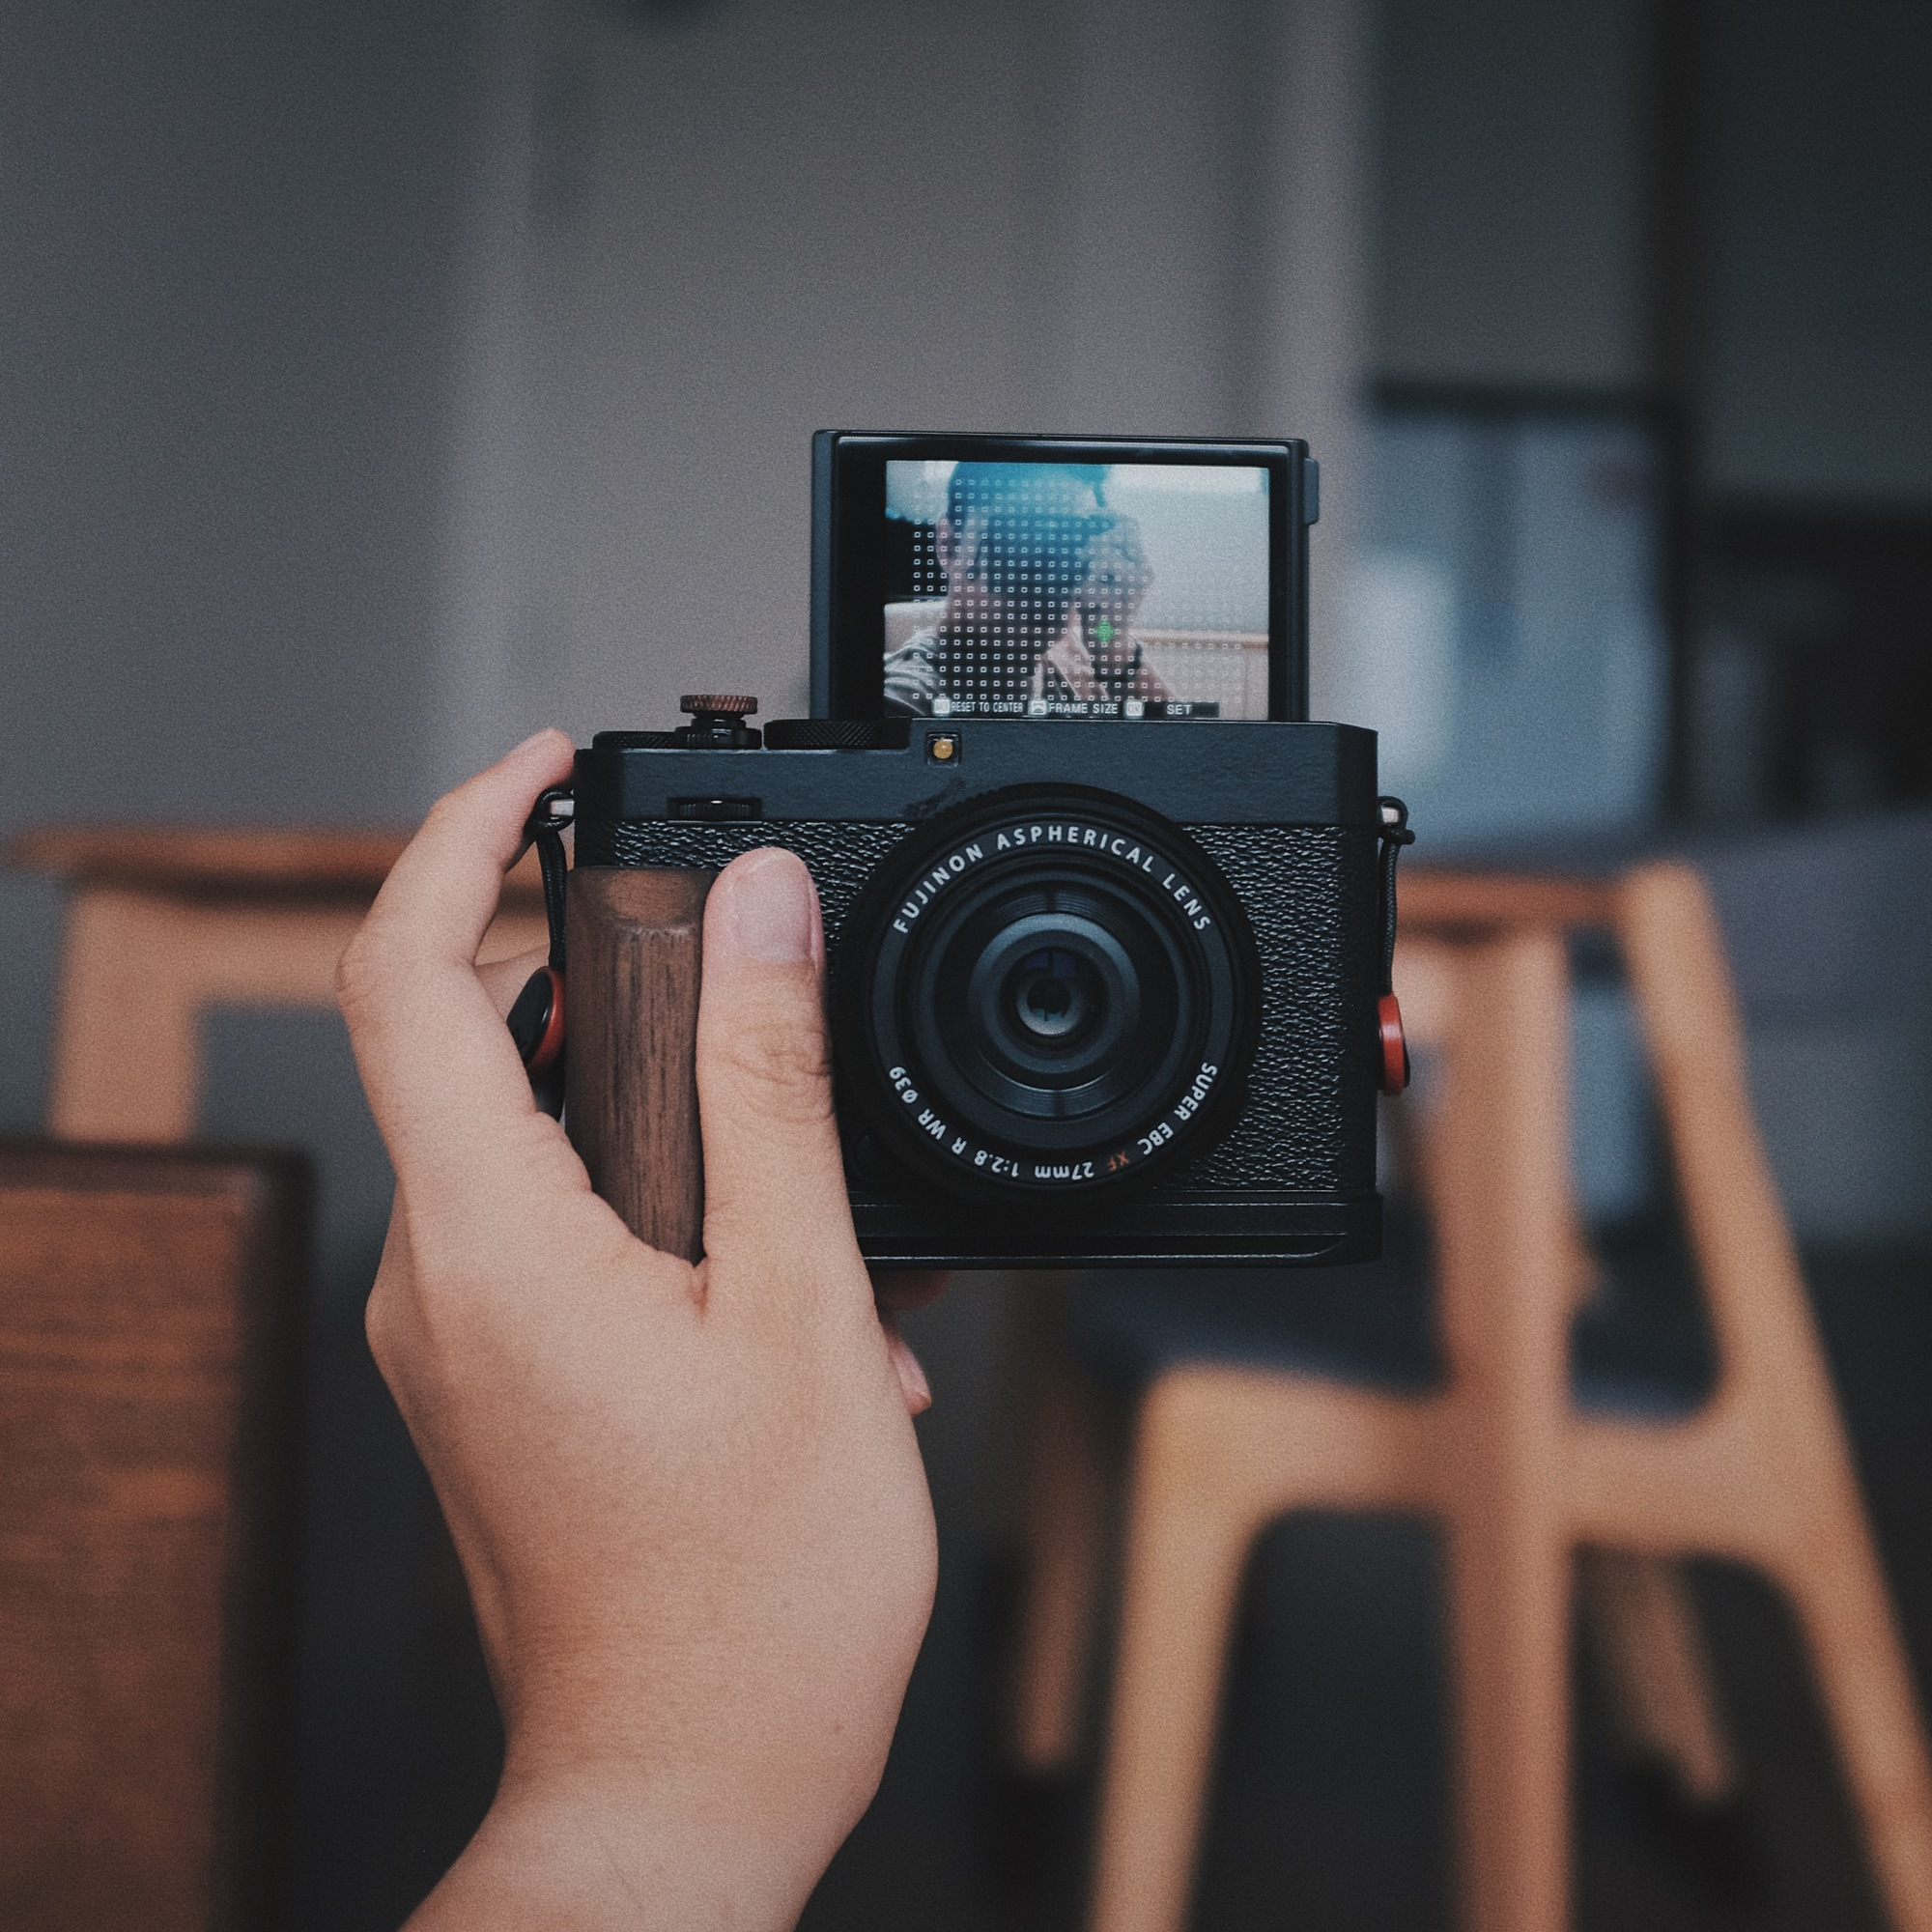
\includegraphics[width=\linewidth]{\envfinaldir/coverpic-prod.jpg}\par
            % \vskip 30pt
            \vfill

            \normalsize\rmfamily\scshape
            \copyright{} The Web Digest Project \hfill\large \envdatestr
        \end{center}
    \end{titlepage}
    % \restoregeometry
}
\newcommand{\simplehref}[1]{%
    \textcolor{blue!80!green}{\href{#1}{#1}}%
}
\renewcommand{\contentsname}{\center\Huge\sffamily\bfseries Contents\par\vskip 20pt}
\newcounter{ipartcounter}
\setcounter{ipartcounter}{0}
\newcommand{\ipart}[1]{
    % \vskip 20pt
    \clearpage
    \stepcounter{ipartcounter}
    \phantomsection
    \addcontentsline{toc}{chapter}{#1}
    % \begin{center}
    %     \Huge
    %     \sffamily\bfseries
    %     #1
    % \end{center}
    % \vskip 20pt plus 7pt
}
\newcounter{ichaptercounter}
\setcounter{ichaptercounter}{0}
\newcommand{\ichapter}[1]{
    % \vskip 20pt
    \clearpage
    \stepcounter{ichaptercounter}
    \phantomsection
    \addcontentsline{toc}{section}{\numberline{\arabic{ichaptercounter}}#1}
    \begin{center}
        \Huge
        \sffamily\bfseries
        #1
    \end{center}
    \vskip 20pt plus 7pt
}
\newcommand{\entrytitlefont}[1]{\subsection*{\raggedright\Large\sffamily\bfseries#1}}
\newcommand{\entryitemGeneric}[2]{
    % argv: title, url
    \parbox{\linewidth}{
        \entrytitlefont{#1}\par\vskip 5pt
        \footnotesize\ttfamily\mdseries
        \simplehref{#2}
    }\vskip 11pt plus 11pt minus 1pt
}
\newcommand{\entryitemGithub}[3]{
    % argv: title, url, desc
    \parbox{\linewidth}{
        \entrytitlefont{#1}\par\vskip 5pt
        \footnotesize\ttfamily\mdseries
        \simplehref{#2}\par\vskip 5pt
        \small\rmfamily\mdseries#3
    }\vskip 11pt plus 11pt minus 1pt
}
\newcommand{\entryitemAp}[3]{
    % argv: title, url, desc
    \parbox{\linewidth}{
        \entrytitlefont{#1}\par\vskip 5pt
        \footnotesize\ttfamily\mdseries
        \simplehref{#2}\par\vskip 5pt
        \small\rmfamily\mdseries#3
    }\vskip 11pt plus 11pt minus 1pt
}
\newcommand{\entryitemHackernews}[3]{
    % argv: title, hnurl, rawurl
    % \parbox{\linewidth}{
    %     \entrytitlefont{#1}\par\vskip 5pt
    %     \footnotesize\ttfamily\mdseries
    %     \simplehref{#3}\par
    %     \textcolor{black!50}{\href{#2}{#2}}
    % }\vskip 11pt plus 11pt minus 1pt
    \begin{minipage}{\linewidth}
            \entrytitlefont{#1}\par\vskip 5pt
            \footnotesize\ttfamily\mdseries
            \simplehref{#3}\par
            \textcolor{black!50}{\href{#2}{#2}}
    \end{minipage}\par\vskip 11pt plus 11pt minus 1pt
}







\begin{document}

\makeheader

\tableofcontents\clearpage




\ipart{Developers}
\ichapter{Hacker News}
\entryitemTwoLinks{An Update on Apple M1/M2 GPU Drivers}{https://news.ycombinator.com/item?id=42011239}{https://lwn.net/SubscriberLink/995383/34dc5950cab5e739/}

\entryitemTwoLinks{Wait Until 8th}{https://news.ycombinator.com/item?id=42011193}{https://www.waituntil8th.org}

\entryitemTwoLinks{Ghost jobs are wreaking havoc on tech workers}{https://news.ycombinator.com/item?id=42010130}{https://www.sfgate.com/tech/article/ghost-jobs-california-tech-industry-19871249.php}

\entryitemTwoLinks{ChatGPT Search}{https://news.ycombinator.com/item?id=42008569}{https://openai.com/index/introducing-chatgpt-search/}

\entryitemTwoLinks{Smashing the Limits: Installing Windows XP in DOSBox-X}{https://news.ycombinator.com/item?id=42008499}{https://fabulous.systems/posts/2023/07/installing-windows-xp-in-dosbox-x/}

\entryitemTwoLinks{Claude for Desktop}{https://news.ycombinator.com/item?id=42007649}{https://claude.ai/download}

\entryitemTwoLinks{Fuzzing between the lines in popular barcode software}{https://news.ycombinator.com/item?id=42006698}{https://blog.trailofbits.com/2024/10/31/fuzzing-between-the-lines-in-popular-barcode-software/}

\entryitemTwoLinks{Sorry, Gas Companies – Parody Isn't Infringement (Even If It Creeps You Out)}{https://news.ycombinator.com/item?id=42006265}{https://www.eff.org/deeplinks/2024/10/sorry-gas-companies-parody-isnt-infringement-even-if-it-creeps-you-out}

\entryitemTwoLinks{Moving to a World Beyond "p < 0.05" (2019)}{https://news.ycombinator.com/item?id=42005635}{https://www.tandfonline.com/doi/full/10.1080/00031305.2019.1583913}

\entryitemTwoLinks{Show HN: TikTok Influencers Database with Analyzed Audio}{https://news.ycombinator.com/item?id=42005516}{https://www.topyappers.com/}

\entryitemTwoLinks{Probability-generating functions}{https://news.ycombinator.com/item?id=42004976}{https://entropicthoughts.com/probability-generating-functions}

\entryitemTwoLinks{SSH Remoting}{https://news.ycombinator.com/item?id=42004206}{https://zed.dev/blog/remote-development}

\entryitemTwoLinks{Hazel: A live functional programming environment featuring typed holes}{https://news.ycombinator.com/item?id=42004133}{https://hazel.org/}

\entryitemTwoLinks{I attended Google's creator conversation event, and it turned into a funeral}{https://news.ycombinator.com/item?id=42002262}{https://www.giantfreakinrobot.com/tech/google-creators-event.html}

\entryitemTwoLinks{Wonder Animation – Video to 3D Animation}{https://news.ycombinator.com/item?id=42001852}{https://adsknews.autodesk.com/en/news/autodesk-launches-wonder-animation-video-to-3d-scene-technology/}

\entryitemTwoLinks{Generative AI Scripting}{https://news.ycombinator.com/item?id=42001811}{https://microsoft.github.io/genaiscript/}

\entryitemTwoLinks{It might be possible to detect gravitons after all}{https://news.ycombinator.com/item?id=42001642}{https://www.quantamagazine.org/it-might-be-possible-to-detect-gravitons-after-all-20241030/}

\entryitemTwoLinks{OpenZFS deduplication is good now and you shouldn't use it}{https://news.ycombinator.com/item?id=42000784}{https://despairlabs.com/blog/posts/2024-10-27-openzfs-dedup-is-good-dont-use-it/}

\entryitemTwoLinks{Hi Google, please stop pooping the bed: a desperate plea from the indie web}{https://news.ycombinator.com/item?id=42000651}{https://build.shepherd.com/p/hi-google-please-stop-the-bed-a-desperate}

\entryitemTwoLinks{NandGame – Build a computer from scratch}{https://news.ycombinator.com/item?id=41999852}{https://www.nandgame.com}\ichapter{Phoronix}
\entryitemGeneric{\hskip 0pt{}AMD EPYC 9655 Benchmarks Show The Terrific Generational Gains With 5th Gen EPYC}{https://www.phoronix.com/review/amd-epyc-9655}

\entryitemGeneric{\hskip 0pt{}AMD Formally Announces Ryzen 7 9800X3D Specs - Should Be Great For Linux Creators}{https://www.phoronix.com/news/AMD-Ryzen-7-9800X3D}

\entryitemGeneric{\hskip 0pt{}Fedora Stakeholders Debate Idea Of "-O3" Optimized Packages}{https://www.phoronix.com/news/Fedora-Debates-O3-Packages}

\entryitemGeneric{\hskip 0pt{}Linus Torvalds Lands A 2.6\% Performance Improvement With Minor Linux Kernel Patch}{https://www.phoronix.com/news/Linus-2.6p-Faster-Scale-Patch}

\entryitemGeneric{\hskip 0pt{}AMX-FP8 Support Upstreamed Into LLVM For Intel Diamond Rapids}{https://www.phoronix.com/news/Intel-AMX-FP8-In-LLVM}

\entryitemGeneric{\hskip 0pt{}SUSE's Agama Installer Adds QR Code To The Console \& Other Improvements}{https://www.phoronix.com/news/SUSE-Agama-10-Installer}

\entryitemGeneric{\hskip 0pt{}SVT-AV1 2.3 Brings More Performance Improvements: AVX-512 \& LTO By Default, More Tuning}{https://www.phoronix.com/news/SVT-AV1-2.3}

\entryitemGeneric{\hskip 0pt{}AMDVLK 2024.Q4.1 Adds A Few More Vulkan Extensions}{https://www.phoronix.com/news/AMDVLK-2024.Q4.1-Released}

\entryitemGeneric{\hskip 0pt{}AMD "Cleaner Shader" Coming For GFX11.0.3 GPUs To Help Ensure User/App Isolation}{https://www.phoronix.com/news/AMD-Cleaner-Shader-GFX11.0.3}\ichapter{Dribbble}
\entryitemGeneric{\hskip 0pt{}Lootbox}{https://dribbble.com/shots/24875582}

\entryitemGeneric{\hskip 0pt{}Internal Universe 🪐✨}{https://dribbble.com/shots/24870294}

\entryitemGeneric{\hskip 0pt{}Gulfstream x theory11 Playing Cards}{https://dribbble.com/shots/24869176}

\entryitemGeneric{\hskip 0pt{}Negative yet Positive Vol.7}{https://dribbble.com/shots/24868890}

\entryitemGeneric{\hskip 0pt{}Onton - Responsive Logo Design}{https://dribbble.com/shots/24866015}

\entryitemGeneric{\hskip 0pt{}Solufacil}{https://dribbble.com/shots/24869750}

\entryitemGeneric{\hskip 0pt{}Raw E}{https://dribbble.com/shots/24869489}

\entryitemGeneric{\hskip 0pt{}Ampersand 3D Logo}{https://dribbble.com/shots/24869500}

\entryitemGeneric{\hskip 0pt{}Rooster}{https://dribbble.com/shots/24854380}

\entryitemGeneric{\hskip 0pt{}cipher}{https://dribbble.com/shots/24855823}

\entryitemGeneric{\hskip 0pt{}"Amphiprion Ocellaris" - Daily art, NFT art}{https://dribbble.com/shots/24854577}

\entryitemGeneric{\hskip 0pt{}Bento Cards v.4 – E-Commerce}{https://dribbble.com/shots/24849627}

\entryitemGeneric{\hskip 0pt{}Neobanking Mobile App Interactions}{https://dribbble.com/shots/24848696}

\entryitemGeneric{\hskip 0pt{}FC Shakhtar Donetsk App. The Concept. Part 2}{https://dribbble.com/shots/24848383}

\entryitemGeneric{\hskip 0pt{}xflow Logo Design - X, Waves}{https://dribbble.com/shots/24847689}

\entryitemGeneric{\hskip 0pt{}The Future has landed ✈️}{https://dribbble.com/shots/24848230}

\entryitemGeneric{\hskip 0pt{}Converse Logo Redesign Concept}{https://dribbble.com/shots/24850036}

\entryitemGeneric{\hskip 0pt{}F Logo}{https://dribbble.com/shots/24850079}

\entryitemGeneric{\hskip 0pt{}ML Fashion 10/10}{https://dribbble.com/shots/24851262}

\entryitemGeneric{\hskip 0pt{}Amplemarket Logo Design}{https://dribbble.com/shots/24843224}

\entryitemGeneric{\hskip 0pt{}Streaming Data}{https://dribbble.com/shots/24838862}

\entryitemGeneric{\hskip 0pt{}It's not a feature, it's a bug}{https://dribbble.com/shots/24844082}

\entryitemGeneric{\hskip 0pt{}Cute Raccoon}{https://dribbble.com/shots/24843120}

\entryitemGeneric{\hskip 0pt{}Nero Code UI concept}{https://dribbble.com/shots/24843816}


\ipart{Developers~~~~(zh-Hans)}
\ichapter{Solidot}
\entryitemGeneric{\hskip 0pt{}龙芯新处理器据报道性能超过了英特尔的 Raptor Lake}{https://www.solidot.org/story?sid=79649}

\entryitemGeneric{\hskip 0pt{}AMD 宣布 Ryzen 7 9800X3D,售价 479 美元 }{https://www.solidot.org/story?sid=79648}

\entryitemGeneric{\hskip 0pt{}俄罗斯表示计划建立替代 Linux 社区}{https://www.solidot.org/story?sid=79647}

\entryitemGeneric{\hskip 0pt{}瑞典和挪威重新考虑无现金社会计划}{https://www.solidot.org/story?sid=79646}

\entryitemGeneric{\hskip 0pt{}2023 年温室气体浓度创新高}{https://www.solidot.org/story?sid=79645}

\entryitemGeneric{\hskip 0pt{}俄罗斯情报机构利用 RDP 发动大规模钓鱼攻击}{https://www.solidot.org/story?sid=79644}

\entryitemGeneric{\hskip 0pt{}Thunderbird for Android 发布首个正式版}{https://www.solidot.org/story?sid=79643}

\entryitemGeneric{\hskip 0pt{}前员工入侵迪士尼乐园餐厅的菜单软件修改过敏信息}{https://www.solidot.org/story?sid=79642}

\entryitemGeneric{\hskip 0pt{}印度对维基百科的诉讼可能产生深远影响}{https://www.solidot.org/story?sid=79641}

\entryitemGeneric{\hskip 0pt{}Valve 要求游戏开发商披露是否使用了内核级反作弊技术}{https://www.solidot.org/story?sid=79640}

\entryitemGeneric{\hskip 0pt{}Google 称其逾四分之一新代码是由 AI 生成的}{https://www.solidot.org/story?sid=79639}

\entryitemGeneric{\hskip 0pt{}Google 搜索排名对独立网站愈来愈不友好}{https://www.solidot.org/story?sid=79638}

\entryitemGeneric{\hskip 0pt{}社区开发者创建 Flutter 分支 Flock }{https://www.solidot.org/story?sid=79637}

\entryitemGeneric{\hskip 0pt{}苹果将 M4 Mac Mini 电源按钮移至底部}{https://www.solidot.org/story?sid=79636}

\entryitemGeneric{\hskip 0pt{}Dropbox 裁员五分之一}{https://www.solidot.org/story?sid=79635}

\entryitemGeneric{\hskip 0pt{}OpenAI 与博通和台积电合作设计 AI 芯片}{https://www.solidot.org/story?sid=79634}

\entryitemGeneric{\hskip 0pt{}X.Org Server 的一个本地提权漏洞存在了 18 年之久}{https://www.solidot.org/story?sid=79633}

\entryitemGeneric{\hskip 0pt{}索尼关闭《星鸣特攻》开发商 Firewalk Studio}{https://www.solidot.org/story?sid=79632}

\entryitemGeneric{\hskip 0pt{}中国三季度智能手机出货量增长 3.2\%}{https://www.solidot.org/story?sid=79631}

\entryitemGeneric{\hskip 0pt{}GitHub Copilot 将支持 Claude 3.5 和 Gemini 模型}{https://www.solidot.org/story?sid=79630}\ichapter{V2EX}
\entryitemGeneric{\hskip 0pt{}[问与答] 5G 消息-运营商努力想回到短信收费的年代...}{https://www.v2ex.com/t/1085537}

\entryitemGeneric{\hskip 0pt{}[美国] 假设这次川普又输了}{https://www.v2ex.com/t/1085536}

\entryitemGeneric{\hskip 0pt{}[问与答] 有没有人和我一样备份聊天记录}{https://www.v2ex.com/t/1085535}

\entryitemGeneric{\hskip 0pt{}[Apple] 月经贴:新 Macmini 内存选择 16、24 还是 32?}{https://www.v2ex.com/t/1085534}

\entryitemGeneric{\hskip 0pt{}[程序员] 为 PVE 搭建一套告警服务}{https://www.v2ex.com/t/1085533}

\entryitemGeneric{\hskip 0pt{}[VPS] 2024 年了,性价比高的海外 vps 求推荐}{https://www.v2ex.com/t/1085532}

\entryitemGeneric{\hskip 0pt{}[问与答] 如何实现分布式消息同步?}{https://www.v2ex.com/t/1085531}

\entryitemGeneric{\hskip 0pt{}[macOS] 如果用 Mac Mini M4 做 Homelab 服务器的话,相比 Linux 需要哪些工具}{https://www.v2ex.com/t/1085530}

\entryitemGeneric{\hskip 0pt{}[问与答] Chatbot 求推荐(附 NextChat / AnythingLLM / Dify 对比)}{https://www.v2ex.com/t/1085529}

\entryitemGeneric{\hskip 0pt{}[iPhone] 16Pro 网络卡顿有解决办法吗}{https://www.v2ex.com/t/1085528}

\entryitemGeneric{\hskip 0pt{}[问与答] 近年来,搜狗输入法的云输入本领是否倒退了?}{https://www.v2ex.com/t/1085527}

\entryitemGeneric{\hskip 0pt{}[问与答] 有什么办法能够 解除 51cto 网站复制 文字 需要登录的限制吗?}{https://www.v2ex.com/t/1085526}

\entryitemGeneric{\hskip 0pt{}[分享发现] nintendo music app coming}{https://www.v2ex.com/t/1085525}

\entryitemGeneric{\hskip 0pt{}[问与答] 🍎Mac Mini M4 能否当作主力机~~~}{https://www.v2ex.com/t/1085524}

\entryitemGeneric{\hskip 0pt{}[互联网] 关于大批量网站监测的需求}{https://www.v2ex.com/t/1085523}

\entryitemGeneric{\hskip 0pt{}[宽带症候群] 为什么家庭宽带不能保持 ssh 连接呢?}{https://www.v2ex.com/t/1085522}

\entryitemGeneric{\hskip 0pt{}[微信] PC 微信 4.0 测试版面向所有人开放,深色模式终于来了}{https://www.v2ex.com/t/1085521}

\entryitemGeneric{\hskip 0pt{}[程序员] [出海记录]开发新手的第 10 个站点上线}{https://www.v2ex.com/t/1085520}

\entryitemGeneric{\hskip 0pt{}[分享发现] 杭州``手机扫描王'' 背信弃义!近 200 份文件瞬间消失,免费用户惨遭坑害!}{https://www.v2ex.com/t/1085517}

\entryitemGeneric{\hskip 0pt{}[路由器] 有 v 友出 gl mt3000 路由器没?}{https://www.v2ex.com/t/1085516}

\entryitemGeneric{\hskip 0pt{}[淘宝] 如何投诉这种无良买家和淘宝平台}{https://www.v2ex.com/t/1085515}

\entryitemGeneric{\hskip 0pt{}[分享发现] [分享] 发现一个不错的数学游戏网站}{https://www.v2ex.com/t/1085514}

\entryitemGeneric{\hskip 0pt{}[VPS] 搬瓦工是不是很久没补货了}{https://www.v2ex.com/t/1085513}

\entryitemGeneric{\hskip 0pt{}[Apple] 准备从日本回来,大佬们买什么能赚回机票}{https://www.v2ex.com/t/1085512}

\entryitemGeneric{\hskip 0pt{}[Apple] 年经贴: mbp 买 14 还是 16}{https://www.v2ex.com/t/1085510}

\entryitemGeneric{\hskip 0pt{}[VPS] 出 1 台阿里云香港轻量云服务器}{https://www.v2ex.com/t/1085509}

\entryitemGeneric{\hskip 0pt{}[Android] 应该选择哪种跨平台方案}{https://www.v2ex.com/t/1085508}

\entryitemGeneric{\hskip 0pt{}[Apple] M4 Mac Mini 512 GB 版本的 SSD 性能比 256 的好么?}{https://www.v2ex.com/t/1085507}

\entryitemGeneric{\hskip 0pt{}[问与答] wechat h5 code 如何桥接多个好友使用呢?}{https://www.v2ex.com/t/1085506}

\entryitemGeneric{\hskip 0pt{}[问与答] nginx 无证书的情况下能否转发 https 流量到另一个 nginx}{https://www.v2ex.com/t/1085504}

\entryitemGeneric{\hskip 0pt{}[杭州] 关于杭州换浙 A 拍照的流程有没有人能讲讲?}{https://www.v2ex.com/t/1085503}

\entryitemGeneric{\hskip 0pt{}[问与答] 各位冲 m4 mbp 的老哥,手头上要是有 m1 的老 mbp,我可以接盘呐}{https://www.v2ex.com/t/1085502}

\entryitemGeneric{\hskip 0pt{}[问与答] 想问下,有没有开源的 android 开发板?}{https://www.v2ex.com/t/1085501}

\entryitemGeneric{\hskip 0pt{}[信息安全] 都說要常換密碼. 我有用 bitwarden/keepass 等等. 但如果每半年換一次 master password 會否很笨?}{https://www.v2ex.com/t/1085499}

\entryitemGeneric{\hskip 0pt{}[Android] flutter 会烂尾么}{https://www.v2ex.com/t/1085497}

\entryitemGeneric{\hskip 0pt{}[问与答] 无人超市的原理是什么?}{https://www.v2ex.com/t/1085496}

\entryitemGeneric{\hskip 0pt{}[分享发现] 非常适合用来直接生成营销内容的新模型}{https://www.v2ex.com/t/1085494}

\entryitemGeneric{\hskip 0pt{}[VPS] 香港服务器}{https://www.v2ex.com/t/1085493}

\entryitemGeneric{\hskip 0pt{}[分享创造] 我单方面认为我们这个产品解决了信息过载问题}{https://www.v2ex.com/t/1085492}

\entryitemGeneric{\hskip 0pt{}[大学] 有没有电气老哥,讲一下现状和人生规划什么的}{https://www.v2ex.com/t/1085491}

\entryitemGeneric{\hskip 0pt{}[分享发现] 分享一些图标制作, ICON 制作, SVG 相关的免费资源}{https://www.v2ex.com/t/1085490}

\entryitemGeneric{\hskip 0pt{}[Go 编程语言] go 程序结构的探讨}{https://www.v2ex.com/t/1085488}

\entryitemGeneric{\hskip 0pt{}[问与答] discord 后台打开相机?不懂}{https://www.v2ex.com/t/1085487}

\entryitemGeneric{\hskip 0pt{}[Mac mini] 新款 Mac mini 的电源键为什么要设计在机身底部?}{https://www.v2ex.com/t/1085486}

\entryitemGeneric{\hskip 0pt{}[C++] CLion 界面字体大小调节问题}{https://www.v2ex.com/t/1085485}

\entryitemGeneric{\hskip 0pt{}[问与答] 刚倒车把别人新车给撞了,报了保险,对方说让我掏钱给她换保险杠。}{https://www.v2ex.com/t/1085484}

\entryitemGeneric{\hskip 0pt{}[酷工作] 广州 | 深圳 | 北京 - 字节跳动 - 前端\资深前端工程师 内推}{https://www.v2ex.com/t/1085483}

\entryitemGeneric{\hskip 0pt{}[分享发现] 分享一个好用的免费落地页(Landing Page)模板}{https://www.v2ex.com/t/1085482}

\entryitemGeneric{\hskip 0pt{}[macOS] mac 升级到最新系统遇到的几个问题,早知道不升级}{https://www.v2ex.com/t/1085481}

\entryitemGeneric{\hskip 0pt{}[旅行] 北京游之天安门,故宫游览心得(个人建议)}{https://www.v2ex.com/t/1085480}


\ipart{Generic News}
\ichapter{AP News}
\entryitemWithDescription{\hskip 0pt{}Bob Costas retiring from baseball play-by-play after 42 years}{https://apnews.com/article/1ce422d7c087c3fc162f4a535fa1f7f0}{}

\entryitemWithDescription{\hskip 0pt{}Rapper Young Thug pleads guilty to gang, drug and gun charges}{https://apnews.com/article/581c38d53dc37f86d5b038f6c23e4b77}{}

\entryitemWithDescription{\hskip 0pt{}`Dances with Wolves' actor is again indicted on sexual abuse charges in Nevada}{https://apnews.com/article/05098564b193d5059aca9d694149c09e}{}

\entryitemWithDescription{\hskip 0pt{}No trick! Halloween temperatures soar above normal in Northeast}{https://apnews.com/article/82c61126a7cc3cc617115db1c54851b0}{}

\entryitemWithDescription{\hskip 0pt{}Film academy adds handwritten `Pulp Fiction' script, Miyazaki art, more to vast collection}{https://apnews.com/article/ca61c46b0919bf6cc534ec804e837ec4}{}

\entryitemWithDescription{\hskip 0pt{}Lawyers are allowed into Giuliani's NYC apartment after he misses a deadline for turning over assets}{https://apnews.com/article/845234e21edd853ca9826ec559fadfbe}{}

\entryitemWithDescription{\hskip 0pt{}John Fisher pledges \$1 billion to construction of A's stadium in Las Vegas}{https://apnews.com/article/0c8240d5e0d555d52f4505ea1e8ecea3}{}

\entryitemWithDescription{\hskip 0pt{}Alex Kirilloff retires from baseball at 26 after an injury-ravaged career with the Twins}{https://apnews.com/article/716e73b3663348b49eab92a690a13cf0}{}

\entryitemWithDescription{\hskip 0pt{}Voting rights groups worry AI models are generating inaccurate and misleading responses in Spanish}{https://apnews.com/article/d4ffabdc006a7c70eece3e28efa3de90}{}

\entryitemWithDescription{\hskip 0pt{}Snow in Hawaii? Cold air and moisture deliver snow to the state's tallest mountain}{https://apnews.com/article/825eff0aeb26919f2fce410ae20e13d1}{}

\entryitemWithDescription{\hskip 0pt{}At 50, Hello Kitty is as `kawaii' and lucrative as ever}{https://apnews.com/article/fb7569605d5e302ddbe92a877fd1768d}{}

\entryitemWithDescription{\hskip 0pt{}Judge sets hearing on \$1M-a-day sweepstakes from Elon Musk PAC helping Donald Trump}{https://apnews.com/article/58e0b42280777b8daa7d4e4f1c6e6514}{}

\entryitemWithDescription{\hskip 0pt{}Game 4 of World Series averages 16.28 million for its most-viewed game since 2019}{https://apnews.com/article/fd8b884c84bf19f5b276d7713da5d25f}{}\ichapter{Reuters}
\entryitemWithDescription{\hskip 0pt{}Trump sues CBS over Kamala Harris interview}{https://www.reuters.com/legal/trump-sues-cbs-over-kamala-harris-interview-2024-10-31/}{Republican presidential candidate Donald Trump sued CBS on Thursday over an interview of his Democratic rival Kamala Harris aired in early October that the lawsuit alleged was "doctored" and misleading, according to a court...}

\entryitemWithDescription{\hskip 0pt{}Egypt denies assisting Israel's military operations amid reports about explosives shipment}{https://www.reuters.com/world/middle-east/egypt-denies-assisting-israels-military-operations-amid-reports-about-explosives-2024-10-31/}{Egypt\textquotesingle s army on Thursday denied it assisted Israeli military operations after media reports that an Egyptian port received a shipment of explosives bound for an Israeli defence...}

\entryitemWithDescription{\hskip 0pt{}Ukraine confident of continued US support after election, says foreign minister}{https://www.reuters.com/world/europe/ukraine-confident-continued-us-support-after-election-says-foreign-minister-2024-10-31/}{Ukraine is confident of continued U.S. support regardless of who wins next week\textquotesingle s presidential election, Foreign Minister Andrii Sybiha said on Thursday, citing what he called strong bipartisan...}

\entryitemWithDescription{\hskip 0pt{}Iraq tries to avoid regional fight as militias fire at Israel}{https://www.reuters.com/world/middle-east/iraq-tries-avoid-regional-fight-militias-fire-israel-2024-10-31/}{Nervously watching Israel\textquotesingle s destructive campaigns in Gaza and Lebanon, Iraq is working to avoid being drawn into the growing regional conflict as Iran-backed armed groups launch attacks on Israel from Iraqi soil, sources...}

\entryitemWithDescription{\hskip 0pt{}Israel, Lebanon make progress on how to implement UN resolution, says Blinken}{https://www.reuters.com/world/middle-east/israel-lebanon-make-progress-how-implement-un-resolution-says-blinken-2024-10-31/}{U.S. Secretary of State Antony Blinken said on Thursday that Israel and Lebanon were moving toward understandings on what is required for implementing a long-violated U.N. resolution that would be the basis for ending the current...}

\entryitemWithDescription{\hskip 0pt{}LaLiga clubs to help raise money for victims of Spain's flash floods}{https://www.reuters.com/sports/soccer/laliga-clubs-help-raise-money-victims-spains-flash-floods-2024-10-31/}{LaLiga and its clubs will help raise funds for the Red Cross to support those affected by the flash floods which have killed at least 158 people in Spain by publicising a campaign during match broadcasts this weekend and through their...}

\entryitemWithDescription{\hskip 0pt{}Iraqi parliament elects Sunni lawmaker al-Mashhadani as speaker, breaking deadlock}{https://www.reuters.com/world/middle-east/iraqi-parliament-elects-sunni-lawmaker-al-mashhadani-speaker-state-news-agency-2024-10-31/}{Iraq\textquotesingle s parliament elected on Thursday Sunni lawmaker Mahmoud al-Mashhadani as its speaker, lawmakers said, breaking a nearly year-long deadlock over the position that had remained vacant due to protracted disagreements...}

\entryitemWithDescription{\hskip 0pt{}Iran preparing strike on Israel from Iraqi territory within days, Axios reports}{https://www.reuters.com/world/middle-east/iran-preparing-strike-israel-iraqi-territory-within-days-axios-reports-2024-10-31/}{Israeli intelligence suggests Iran is preparing to attack Israel from Iraqi territory in the coming days, possibly before the U.S. presidential election on Nov. 5, Axios reported on Thursday, citing two unidentified Israeli...}

\entryitemWithDescription{\hskip 0pt{}Mexico's Sinaloa bans Halloween costumes amid cartel violence}{https://www.reuters.com/world/americas/mexicos-sinaloa-bans-halloween-costumes-amid-cartel-violence-2024-10-31/}{In the Mexican state of Sinaloa, authorities have ordered residents not to don masks or costumes on Thursday night for Halloween to avoid being confused with criminals amid a worsening cycle of cartel...}

\entryitemWithDescription{\hskip 0pt{}Blast kills man in apartment in Greek capital; anti-terrorism probe launched}{https://www.reuters.com/world/europe/blast-kills-man-apartment-greek-capital-anti-terrorism-probe-launched-2024-10-31/}{A man was killed and a woman was seriously hurt in an explosion in an apartment in the Greek capital Athens on Thursday and an anti-terrorism investigation was underway, the fire brigade and police officials...}

\entryitemWithDescription{\hskip 0pt{}Georgian opposition calls for more protests as exit pollster says official result 'impossible'}{https://www.reuters.com/world/europe/georgian-opposition-calls-street-protests-exit-pollster-says-official-result-2024-10-31/}{Three Georgian opposition parties who allege last weekend\textquotesingle s election was rigged called for streets protests next Monday as an exit pollster said the official result, which gave victory to the ruling Georgian Dream party...}

\entryitemWithDescription{\hskip 0pt{}US says 8,000 North Korean troops in Russia's Kursk}{https://www.reuters.com/world/europe/us-says-8000-north-korean-troops-russias-kursk-2024-10-31/}{The United States has received information that indicates that "right now" there are 8,000 North Korean troops in Russia\textquotesingle s Kursk region, deputy U.S. Ambassador to the United Nations Robert Wood told the Security...}

\entryitemWithDescription{\hskip 0pt{}Zelenskiy blasts allies for 'zero' response to North Korean deployment}{https://www.reuters.com/world/europe/ukraines-zelenskiy-blasts-allies-zero-response-nkorean-deployment-2024-10-31/}{President Volodymyr Zelenskiy said a weak reaction would encourage Russia\textquotesingle s Vladimir Putin to beef up the...}






\clearpage
\leavevmode\vfill
\footnotesize

Copyright \copyright{} 2023-2024 Neruthes and other contributors.

This document is published with CC BY-NC-ND 4.0 license.

The entries listed in this newsletter may be copyrighted by their respective creators.

This newsletter is generated by the Web Digest project.

The newsletters are also delivered via Telegram channel \CJKunderline{\href{https://t.me/webdigestchannel}{https://t.me/webdigestchannel}}.\\
RSS feed is available at \CJKunderline{\href{https://webdigest.pages.dev/rss.xml}{https://webdigest.pages.dev/rss.xml}}.

This newsletter is available in PDF at
\CJKunderline{\href{https://webdigest.pages.dev/}{https://webdigest.pages.dev/}}.

The source code being used to generate this newsletter is available at\\
\CJKunderline{\href{https://github.com/neruthes/webdigest}{https://github.com/neruthes/webdigest}}.

This newsletter is also available in
\CJKunderline{\href{http://webdigest.pages.dev/readhtml/\envyear/WebDigest-20241101.html}{HTML}} and
\CJKunderline{\href{https://github.com/neruthes/webdigest/blob/master/markdown/\envyear/WebDigest-20241101.md}{Markdown}}.


\coverpic{https://unsplash.com/photos/a-man-in-a-suit-and-tie-standing-in-front-of-a-swimming-pool-kgUjBw0fOYI}{Bennie Bates}


\end{document}
